% ----------------------------------------------------------------------------%
%                                   XeLaTeX                                   %
% ----------------------------------------------------------------------------%

\documentclass[journal,a4paper,12pt]{IEEEtran}

\usepackage[utf8]{inputenc}
\usepackage{graphicx}
\usepackage{subfigure}
\usepackage{xspace}

\graphicspath{{./img/}}

\newcommand*{\LEGO}{
\includegraphics[height=8pt]{lego.png}\xspace}
\newcommand*{\NXT}{
\includegraphics[height=8pt]{nxt.png}\xspace}
\newcommand*{\LEJOS}{
\includegraphics[height=8pt]{lejos.png}\xspace}
\newcommand*{\degree}{\ensuremath{^\circ}\xspace}

\title{Group 5 Final Report}
\author{Andrius Sutas, Caith\'{a}n Moore, Clemens Wolff, Sarah McGillion, Jona Duka, Jamie Ironside, Ozg\"{u}r Osman, Christopher Rooney, Alexander Pantov}
\markboth{System Design Project 2012/13}{}

\begin{document}
\maketitle


\section{Introduction}\label{s:introduction}

Group 5, also known as HSTYA (``Holly So Three Years Ago''), named itself after ``Holly'', one of the most successful robots in the history of the System Design Project; an open proclamation and constant reminder of the aim of the group: settle for no less than a victory on the final day tournament.

In order to make this ambition reality, all nine members of our group leveraged their experience and expertise to the fullest extent --- while still remaining free to work on goals aligned with their interests, at their own speed, and using their own paradigms. Section \ref{s:team} explains how we achieved this task of minimising ceremony while maximising productivity.

From early on our group manufactured novel solutions to problems ranging from motion algorithms to hardware kicker design to communication protocols --- it was thus clear that our ambition was not misguided. Section \ref{s:robot} presents our innovations and gives a summary introduction to the design process behind our robot.

The group's performance was a result of the interplay of a multitude of factors --- chiefly among them the ability to fail early, fail often, and learn from these failures. Section \ref{s:conclusion} concludes this report by giving a meditation on the lessons learned over the course of our robot implementation process.


\section{Team Dynamics}\label{s:team}

\begin{figure}[!htb]
\centering
  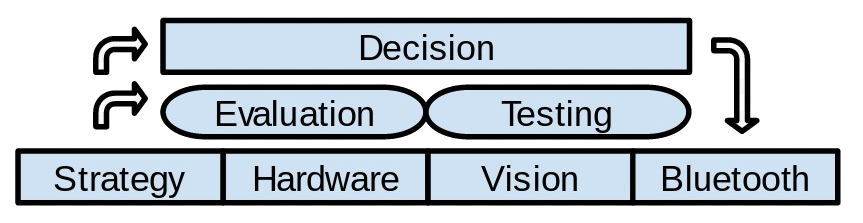
\includegraphics[width=\columnwidth]{organisation.png}
  \caption{Team organisation}
  \label{f:organisation}
\end{figure}

Our group consisted of people with very diverse backgrounds, skills, interests, and motivations. In order to avoid any possible problems that might arise from the incompatibilities inherent in such a mix, we opted against rigorous process and in favour of a largely self-directed and motivation-based environment.

The group collectively split the robot design process into several sub-problems. Every member then weighted their skills against their interests in selecting which sub-problem specific group they chose to join. Attempting to minimise ceremony, each group was independent in how it structured its internal workings and was not required to give regular progress reports.

In an effort to aggregate experience gained in each sub-group, testing and evaluation were undertaken collectively. The results of these, along with feed-in from the team-manager --- providing a birds-eye-view on the project due to being intimately familiar with the workings of each sub-group --- were used to  collectively take high-level decisions.

Figure \ref{f:organisation} summarises the resulting organisational structure.

The choice of this scheme was validated in three ways. Firstly, attempts at introducing more defined inter-group communication protocols such as regular on-the-fly status updates, or more rigorous intra-group planning mechanisms such as formally defined deliver-by dates turned out to add more managerial overhead than they added in value for such small a team with existing short communication channels. Secondly, our group did not have any instances of duplicate or incompatible work, or capacities being left idle, pointing towards our scheme being efficient at allocating talent and resources. Thirdly, our interest-based job-division process meant that everyone was working on tasks personally interesting to them, leading to high motivation. Many people went above and beyond what could have been expected of any student. This manifested itself in a spectrum ranging from organising rotas in order to maximise the time spent on the robot to sleeping in the laboratories after working way too late for too many days in a row.

While sub-groups --- and indeed, individuals --- were independent in how they organised their work, pair programming was heavily advocated and widely up-taken. The benefits of this technique can not be overstated: more concise code, less obscure program logic, fewer bugs, shorter modules, peer-learning, and most importantly elimination of the single point of failure where only one group member is familiar with a particular task leading to all development efforts rising and falling with that individuals availability and involvement --- which might not be synchronised with the demands of the project.


\section{Robot Design}\label{s:robot}

Analysis of past System Design Projects' robots led our group to the insight that the key factors consistently leading to success are mobility, agility, and speed. Further investigation revealed that there are only two ways to realise all three of these requirements: lightweight differentially-steered robots and holonomic robots. The former has the advantage that its basic functionality is largely trivial to implement in both hardware and software. However, due to the limitations inherent in two-wheeled propulsion, such a robot necessitates a sophisticated movement strategy and is not very error tolerant. The omnidirectional approach is more complex to build and requires some relatively advanced control theory to manipulate. However, it also provides an edge in agility due to enabling the direct control of three degrees of freedom on the plane. This makes the implementation of strategies straight-forward and thus reduces the overhead and number of points-of-failure later in the robot design process. Confident in our abilities to lay a solid holonomic foundation, we decided to embark on a journey down the later path.

\begin{figure}[!htb]
\centering
  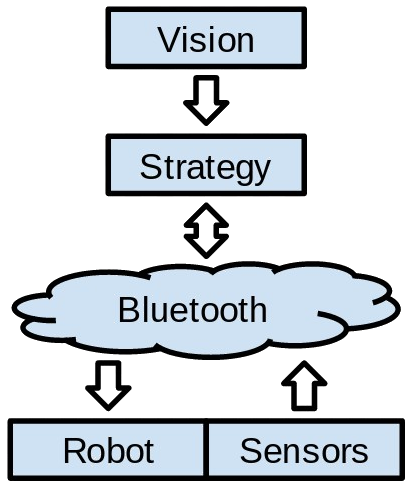
\includegraphics[width=0.5\columnwidth]{architecture.png}
  \caption{High-level robot architecture}
  \label{f:architecture}
\end{figure}

From an architectural point of view, analysis of the robots of previous System Design Project generations revealed that the structure shown in Figure \ref{f:architecture} enjoys wide-spread acceptance. After brief deliberation, we did not see any reason to deviate from this framework. The following sections describe our implementation of each of the sub-components in Figure \ref{f:architecture} in detail. Section \ref{s:hardware} introduces the physical design --- the ``body'' --- of our robot. The vision system, our robot's ``eyes'', is presented in Section \ref{s:vision}. Section \ref{s:strategy} shows how our robot's ``brains'' turn vision inputs into plans for the physical robot to execute. Section \ref{s:communications} provides a synthesis of our architecture's workings by explaining how the various sub-modules inter-operate, with a specific focus on our handling of the hardware-software interface problem.


\subsection{Hardware}\label{s:hardware}

There are two ways to implement holonomic locomotion, both of them relying on a specific positioning of omnidirectional wheels around the central axis of the robot: three wheels separated by 120\degree angles, or four wheels separated by 90\degree angles. The former requires less hardware --- one fewer wheel and motor --- but its geometry is awkward to implement in \LEGO, the hardware of choice for this project, which is why the group decided to go with the later design. Figure \ref{f:wheels} shows the finished implementation of the concept. A square frame ensures that the wheels are positioned equidistantly. Close proximity of the wheels to the frame edge helps with stability.

\begin{figure}[!htb]
\centering
  \subfigure[Side view]{
    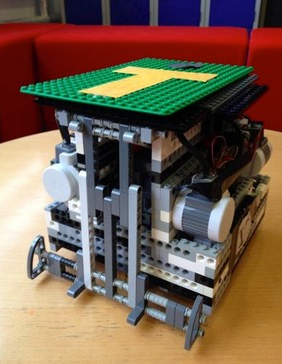
\includegraphics[height=5cm]{holly_final.png}
    \label{f:holly}}
  \subfigure[Bottom view]{
    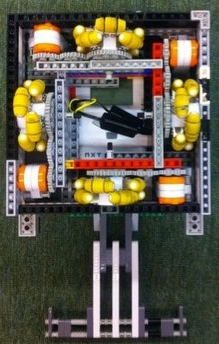
\includegraphics[height=5cm]{holly_bottom.png}
    \label{f:wheels}}
  \caption{Main development effort: our holonomic robot}
  \label{f:robot}
\end{figure}

Each wheel is connected to a motor via a gear train. This allowed us to test different gear ratios with ease in order to determine the optimal balance between torque and speed. Higher speed allows a faster approach and dribbling; higher torque protects the robot from being pushed by the opponent. Our testing covered all sensible combinations of the seven types of gears available to us and revealed that a ratio of 24:40 provided the best speed-torque trade-off.

The frame being square in shape left us with ample space in the centre of the robot for its minicomputer --- a \NXT brick running the operating system \LEJOS. The minicomputer is quite heavy compared to the rest of the robot; our initial attempts to fit the computer sideways onto the robot were therefore suboptimal: they biased the load-balance to one side, resulting in slanted straight-line motion. This was fixed by placing the minicomputer horizontally, with its control display facing towards the wheels as shown in Figure \ref{f:wheels}. This provided easy access for computer-restarts and equipped the robot with a low gravitational centre. The later, coupled with the symmetry of our design, gave the robot an even weight distribution, further increasing its stability.

Our main innovation in hardware terms was our kicker. Implementing the crank mechanism depicted in Figure \ref{f:crank} allowed us to transfer the kickers motors rotary motion to linear motion which is much more appropriate to the task of transferring energy to a ball. This design change doubled our kick potential and allowed us to score from anywhere on the pitch, where our previous naive implementations only propelled the ball about one-half pitch length. Figure \ref{f:prongs} shows that we placed prongs on the sides of the kicker. This allowed us to maintain control of the ball while strafing --- the main mode of locomotion of holonomic robots.

\begin{figure}[!htb]
\centering
  \subfigure[Mechanism\protect\footnotemark]{
    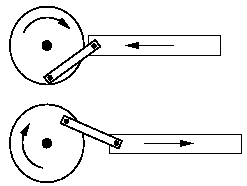
\includegraphics[width=0.45\columnwidth]{crank.png}
    \label{f:crank}}
  \subfigure[Implementation, side view]{
    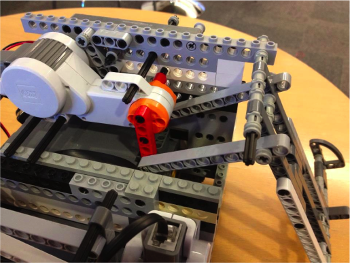
\includegraphics[width=0.45\columnwidth]{crank_kicker.png}
    \label{f:prongs}}
  \caption{Crank kicker design}
  \label{f:kicker}
\end{figure}
\footnotetext{Figure credit: J. Young, ``Simple Machine Elements'', retrieved from www.cnx.org/content/m13594/ on 25 April 2013}

Figure \ref{f:holly} shows our design in its entirety. In order to validate our choices, we built the two differentially-steered  robots in Figure \ref{f:other_robots}. The robot in Figure \ref{f:newbot} was very lightweight and therefore had a high top-speed. However, when pitching it against our holonomic robot, the later consistently scored more goals due to not having to slow down and spend time to turn. The robot in Figure \ref{f:dummybot} was remotely controlled to allow us to test our holonomic approach against a human opponent --- and therewith against an optimal differentially-driven strategy.

\begin{figure}[!htb]
\centering
  \subfigure[Sparring robot]{
    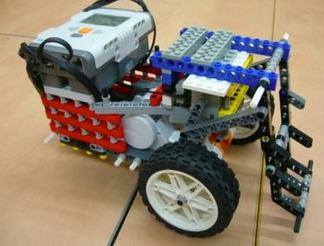
\includegraphics[height=3cm]{robot_dummy.png}
    \label{f:dummybot}}
  \subfigure[Alternative lightweight robot]{
    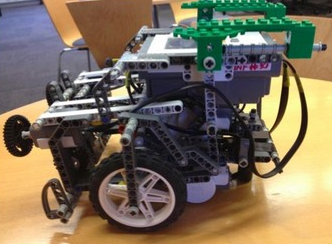
\includegraphics[height=3cm]{robot_new.png}
    \label{f:newbot}}
  \caption{Secondary development efforts}
  \label{f:other_robots}
\end{figure}


\subsection{Vision}\label{s:vision}

The task of the vision-subsystem is to take raw data from the camera observing the robots and ball during play and extract from it information such as positions, velocities and accelerations. The main challenges in this domain are building robustness to changes in scene illumination and handling the noisiness of the real world.

Since a robust solution to this transduction problem is essential to a team's performance in all aspect of the System Design Project, we chose to focus on re-using code from vision systems of groups successful in previous years. As when using any sort of legacy application, this presented us with two main challenges: difficulty integrating a component from a software system designed in a different way from ours and the lack of a deeper knowledge of the appliance being used leading to inertia against fixing bugs and improving the system's performance.

We tackled the integration problem by encapsulating the vision system's responsibilities into a service. This service --- rather than the vision system directly --- was then queried for information, thusly making us agnostic to the underlying implementations and allowing us to try different systems easily. The resulting clear separation of concerns also helped with solving the second legacy-system-integration challenge outlined above: upon realising any deficiencies in some vision package, we could simply swap it out for another rather than having to invest time into understanding a completely foreign piece of software and attempting to fix bugs in it. Being able to try out six different vision systems over the course of the System Design Project, while only spending an aggregate three man-days on the task, points towards the effectiveness of this scheme.

At the start of the System Design Project, we searched for a vision package that was easy to get running and settled on the 2012 implementation by Group 5. This pragmatic consideration allowed the team to focus on more pressing concerns, such as implementing milestone relevant functionality; its pay off was soon evident: at any point in time we were developing functionality for at least one milestone in advance.

After finalising the bulk of our robot's functionality, we focused on finding a more robust alternative to our first quick-and-dirty vision-choice --- which had long since started to show its weakness in coping with a wide range of lighting conditions leading to difficulties in detecting the yellow robot and loosing track of the ball in shadowy areas of the pitch. After trying a number of different vision systems from groups in 2011 and 2012, we identified the 2012 implementation of Group 9 and the 2011 implementation of Group 5 as the two most promising candidates. The former implemented Kalman filtering. The later tracked objects based on region properties rather than color. Both were able to compensate for the loss of some object in a frame by predicting its features from past information. Both worked admirably in almost all situations. We chose to use the later system because, by design, it was more robust to extreme situations such as spectators interfering with the camera or objects being lost by the robots.


\subsection{Strategy}\label{s:strategy}

The strategy-subsystem lies at the intersection of vision and hardware. It analyses inputs from the former to communicate plans to the later. Its main tasks: shooting and defending penalties and enabling the robot to score goals while preventing the opponent from doing the same.

Our strategy for both penalty modes was straight-forward. To defend, our robot moves to the intersection of the goal line and a line drawn from the attacking robot into the direction it is facing. A trivial geometric argument shows that this maximises the chance of intercepting the opponent's kick. We later added the constraint that our robot should not move out of the goal limits, even if the opponent is facing that way. This required being able to execute accurate movements and being able to detect the orientation of the enemy with high precision --- and therefore was not perfected until we switched to the more reliable vision system. To shoot a penalty, our robot simply kicks as fast as possible. This strategy was chosen for two reasons: firstly, our movement routines would not allow us to reliably turn in place to face the most exposed part of the opponent's goal, secondly, the other robots were simply too fast to respond to our movements --- we thus had better chances of scoring if we kicked as soon as possible, in order to potentially take the other robot unaware.

While the bulk of our penalty-strategy was finalised relatively soon, our strategy for open play evolved quite a lot from its initial inception for the first friendly tournament to its ultimate test on the final day. At first, we decided that the situations the robot would find itself in during the matches --- being in possession of the ball, the enemy being in possession of the ball and close to or distant from our goal, no robot having control of the ball, etc. --- demanded quite distinct behaviours. An implementation of such a strategy depended on keeping track of a multitude of internal states and planning for different contingencies. This turned out to be overly complex and therefore both hard to implement and error prone, leading to our unsatisfactory performance in the first two friendly tournaments.

Our saving grace was the realisation that all of these cases can be condensed to just one. Simply getting behind the ball as fast as possible while always facing the opponent's goal naturally leads to a strong offence and defense: being behind the ball positions our robot between the enemy and our goal enabling us to use our bulky hardware to deflect any attempted shots; perpetually facing the opponent's goal leads to many opportunities to score. Our strategy implementation was thus simple: when in possession of the ball, dribble to the enemy goal and shoot whenever the likelihood of scoring --- measured as a function of distance and angle to the goal --- is high enough, when not, move towards the ball. Note that this strategy can only be implemented in holonomic robots since their additional degree of freedom is what makes the continuous facing of the opposing goal possible in the first place.

Scoring more goals during the third friendly tournament than in the previous two combined increased our confidence in the soundness of our theory. Fixing minor implementation details allowed us to win the final day without conceding a single match --- the ultimate validation of our strategy.


\subsection{Communications}\label{s:communications}

All of our clever strategies and innovative hardware design would have been for nought if we could not have been able to reliably make the two communicate --- from the beginning it was clear that we needed a sure-fire way of sending control commands to our robot. With this in mind the communications task was given high priority. A number of final reports from previous years noted issues with Bluetooth connectivity --- so instead of reusing broken code we decided to re-implement it ourselves, despite our group's aversion against duplicating previously implemented efforts. Building a communications protocol from scratch meant pouring through \LEJOS and Bluetooth documentation, but had the benefit of our group gaining a full understanding of vital Bluetooth implementation details such as limited message queue sizes. Our efforts were not in vain: over the entire course of the project, we did not have a single Bluetooth failure.

Our protocol is based on a request-reply architecture. A request is a byte array sent from the computer hosting the strategy to the robot. The first byte is an opcode representing a possible action like ``kick'' or ``set motor speeds'', the following bytes specify additional opcode-specific parameters (e.g. four numbers indicating motors speeds). Upon receiving such a request, the robot immediately replies with an acknowledgement specifying whether or not it was able to understand the last command. With each such reply, the robot also reports back the state of its touch sensors, enabling collision-detection and -handling in the strategy-layer. This architecture allowed us to update robot control around 10 times per second.

Alternatively, we could have kept the robot in receive-only mode and flood it with commands. This doubles the refresh rate, but leads to unpredictable side-effects. For example, we would not know if a kick command send to the robot actually reached it, or if it was dropped due to queue size limits or similar issues. Since one of our main design principles was to maximise reliability, we discarded this design.


\section{Lessons learned and conclusions}\label{s:conclusion}

Our team met the goal we set out for ourselves in the initial meeting: we won the competition and consistently delivered top-of-the-class results during the milestones. This was achieved through the smooth, cohesive working of our group, as well as the high quality and innovative component of our individual contributions --- enabled by strong communication, motivation and collaboration at each step of the process.

Our dearly acquired lessons for future System Design Project generations are:
\begin{itemize}
\item Collaboration, cooperation and support from team members is crucial to the success both as a team and as an individual.
\item Document changes extensively so that whoever picks up your code can contribute better.
\item Build highly generalised methods that cover more than just your current specification. The specifications will change, and the time saved in reimplementation will outweigh the time taken to code a general solution in the first case.
\item Make sure that more than one person understands each section. Failure to do so will lead to key components of your system not working when that person is not around.
\item Don't be scared of re-factoring and throwing away large chunks of your system. If there is a simpler way to do a certain task, it will be easier to understand and maintain. With good version control, any ``bad'' edits can be reverted easily.
\item Commit often to your revision control system. With small updates, you can easily identify problems and roll back to a specific point. With large updates, you are more likely to lose lots of good work to undo small bad changes.
\end{itemize}

\end{document}
